\documentclass{article}

\usepackage{arxiv}
\usepackage{hyperref}       % hyperlinks
\usepackage{url}            % simple URL typesetting
\usepackage{booktabs}       % professional-quality tables
\usepackage{amsmath}        % AMS math extensions
\usepackage{amsfonts}       % blackboard math symbols
\usepackage{microtype}      % microtypography
\usepackage{graphicx}
\usepackage{mathptmx}
\usepackage{tikz}
\usepackage{indentfirst}
\usepackage{setspace}
\usepackage[12pt]{extsizes}
\usetikzlibrary{shapes,arrows}
\usetikzlibrary{calc,decorations.pathmorphing}
\usepackage{subcaption}
\usepackage{float}
\usepackage{enumitem}

\setlength{\floatsep}{0pt}
\setlength{\textfloatsep}{0pt}
\setlength{\intextsep}{0pt}
\setlist{noitemsep, topsep=0pt}

% \doublespacing

% for bibliography
\usepackage[backend=biber,hyperref=true,style=numeric,bibencoding=utf8]{biblatex}
\addbibresource{refs.bib}

% use parindent together with parskip
\setlength{\parindent}{2em}

\title{Exposure Estimation Exploration}
\author{
    \textbf{Aaron Yagnik} \\
    Cornell University \\
    \texttt{ay294@cornell.edu}
    \and
    \textbf{Aspen Smith} \\
    Cornell University \\
    \texttt{acs378@cornell.edu}
    \and
    \textbf{Timothy Vu} \\
    Cornell University \\
    \texttt{tv75@cornell.edu}
}

\vspace{-1em}
\date{\today}
\renewcommand{\undertitle}{}
\renewcommand{\headeright}{}

\usepackage{titlesec}
\titlespacing*{\section}{0pt}{\parskip}{0.5em}

\begin{document}

\maketitle
\noindent \textit{Project GitHub Repository Hyperlink: }\href{https://github.com/asmith236/cs6850-exposure-estimation}{cs6850-exposure-estimation} 
\section*{Introduction} 

Exposure estimation in networks plays a crucial role in understanding how information propagates across populations, influencing areas such as public health, tracking misinformation, and social media moderation. In the context of public health, for instance, accurately estimating exposure to critical information (i.e., vaccine campaigns or disease prevention strategies) can help allocate resources effectively. Similarly, in the realm of social media moderation, identifying the extent to which harmful or false information spreads enables platforms to take targeted action. However, the inherent complexity and massive scale of online social networks make direct measurement of exposure both technically challenging and computationally intensive. 

In this exploration, we base most of our initial foundational concepts on the paper ``Estimating Exposure to Information on Social Networks" \cite{10.1145/3688599}, by Nettasinghe et al., which tackles the challenge of measuring how much of a network has been exposed to specific information. They proposed two methods: a simple ``vanilla" estimator and a friendship paradox-based estimator, which leverages the principle that people’s friends are often more connected than they are, to improve exposure estimation accuracy in networks with highly connected hubs. The paper ``The Generalized Friendship Paradox: An Analytical Framework" \cite{fotouhi2014generalizedfriendshipparadoxanalytical}, authored by Fotouhi et al., builds on the friendship paradox by including ``quality" as a factor in network growth. In this context, the quality of a node refers to an intrinsic value or attribute associated with the node, such as the reliability, influence, or significance of the information it shares. For example, in a social network, quality may represent a user's credibility, content value, or popularity. Higher-quality nodes are more likely to influence network behavior, as their content is more widely shared or regarded as more impactful. Together, these papers offer valuable insights into estimating information flow across various network types, accounting for different structural and measurement challenges.


We build upon the Nettasinghe et al. and Fotouhi et al. papers by proposing two estimators of our own. First, we propose a hybrid estimator, \( \hat{f}_H \), which combines the benefits of both paper findings by dynamically adjusting the weighting for nodes based on their degree. Secondly, we propose the Fotouhi estimator, \( \hat{f}_F \), which factors node quality into the estimation, weighs neighbor contribution, and corrects for quality-distribution biases.

\section{Related Work}

This section presents and explains concepts derived in the two aforementioned papers, Nettasinghe et al. \cite{10.1145/3688599} and Fotouhi et al. \cite{fotouhi2014generalizedfriendshipparadoxanalytical}. These concepts are at the core of the hybrid and Fotouhi estimators we propose in section 2.

\subsection{Vanilla Estimator} 

The vanilla method, proposed by Nettasinghe et al., involves uniform sampling across the network to randomly select nodes. From there, it determines each node's exposure status based on the shared content of their neighbors. Nettasinghe et al. explicitly defines the vanilla method as follows:

After sampling \( n \) random nodes \( X_1, \ldots, X_n \) uniformly and independently from the set of all nodes \( V \), the following equation can be used to estimate the true average exposure, \( \bar{f} \):

\begin{equation}
\hat{f}_{\text{V}} = \frac{\sum_{i=1}^n f(X_i)}{n}
\label{eq:vanilla_estimate}
\end{equation}

The function \( f(Y_i) \) in this equation represents the exposure status of the sampled node \( X_i \). Specifically, \( f(Y_i) \) is a binary indicator variable, where \( f(Y_i) = 1 \) if node \( Y_i \) has been exposed to the information being estimated and \( f(Y_i) = 0 \) if it has not. This binary nature reflects the concept of exposure in the context of the problem: a node either has or has not encountered the information.

While the vanilla method approach is simple and unbiased (\(\mathbb{E} \left\{ \hat{f}_{V1} \right\} = \bar{f}\)), it often yields exposure estimation results with high variance, especially in cases where the information-sharing pattern is sparse or concentrated in particular clusters. This method is used as the baseline for the experiments conducted in Nettasinghe et al. regarding the friendship paradox-based method, which is highlighted in the next section.

\subsection{Friendship Paradox and Friendship Paradox-Based Estimator}

\subsubsection{Friendship Paradox}

The friendship paradox is a graph-theoretic phenomenon that highlights an intuitive yet mathematically significant observation about networks: on average, the friends of a randomly selected individual are likely to have more friends than the individual. This paradox is formally described as follows:

\noindent\textit{Friendship Paradox Theorem:} Consider an undirected graph \( G = (V, E) \), where \( V \) is the set of nodes and \( E \) is the set of edges. Let \( X \) be a node sampled uniformly at random from \( V \), and \( Y \) be a node sampled uniformly as the endpoint of a randomly sampled edge \( e \in E \). Then, the expected degree of \( Y \) satisfies:
\[
\mathbb{E}\{d(Y)\} \geq \mathbb{E}\{d(X)\},
\]
where \( d(X) \) and \( d(Y) \) denote the degrees of nodes \( X \) and \( Y \), respectively.

In simpler terms, the theorem states that a randomly chosen friend (node \( Y \)) is more likely to have a high degree (i.e., many connections) compared to a randomly chosen individual (node \( X \)). This occurs because high-degree nodes appear as neighbors to more nodes, making them more likely to be sampled when choosing a random edge.

The friendship paradox has important implications for network sampling, as it allows for the selection of high-degree nodes without prior knowledge of the network structure. Sampling random friends (endpoints of edges) helps identify influential nodes efficiently, which is particularly useful for problems involving information dissemination or exposure estimation.

\subsubsection{Friendship Paradox-Based Estimator}

Building upon the friendship paradox, Nettasinghe et al. proposes the friendship paradox-based estimator to estimate the average exposure, \( \bar{f} \), across an information network. This method leverages the observation that high-degree nodes are more likely to be sampled when selecting random friends, thus reducing variance compared to uniform sampling. After sampling \( n \) random friends \( Y_1, \dots, Y_n \) from the network independently, where each \( Y_i \) is selected as a random end of a random link (i.e., one end of a uniformly sampled edge), the friendship paradox-based estimator estimates the average exposure \( \bar{f} \) using the following equation:
\[
\hat{f}_{\text{FP}} = \frac{\bar{k}}{n} \sum_{i=1}^n \frac{f(Y_i)}{d(Y_i)},
\]
where \( \bar{k} \) is the average degree of the graph, \( d(Y_i) \) is the degree of the sampled friend \( Y_i \), and \( f(Y_i) \) denotes whether \( Y_i \) has been exposed to the information (taking a value of 0 or 1).

The friendship paradox-based estimator employs non-uniform sampling by targeting 'friends' (connections) of randomly selected nodes. This approach biases the sampling process toward high-degree nodes, which are more influential in information spread. Nettasinghe et al. demonstrates through simulations on both synthetic and real-world networks that this method consistently outperforms the vanilla estimator in terms of accuracy and variance, particularly in centralized network structures where degree correlations align.

By leveraging the friendship paradox, this method effectively reduces estimation error and variance, making it well-suited for networks with skewed degree distributions, such as scale-free or social networks.

\subsection{Network-Level Quality Paradox (NQP)} 

The Network-Level Quality Paradox (NQP) extends the friendship paradox to account for node quality. Although the friendship paradox states that the neighbors of a node are, on average, more connected than the node itself, the NQP highlights that the neighbors of a node can also be of higher quality on average. This phenomenon is particularly clear in networks where high-quality nodes (i.e., influential individuals or authoritative accounts) are also highly connected, increasing their role in information spread.

To address this, Fotouhi et al. introduces the NQP correction factor, \( 1 + \text{NQP} \), which adjusts for the over representation of high-quality nodes in neighbor-based sampling. This correction ensures that exposure estimators do not overestimate the contribution of these nodes to the overall exposure. The correction is particularly important in networks with a strong positive correlation between degree and quality, where ignoring the NQP can lead to significant bias in exposure estimates.

The NQP correction also accounts for the interaction between quality and network structure on a global scale. In highly centralized networks, where a small subset of nodes dominates the flow of information, the NQP ensures that exposure estimates remain unbiased by scaling the influence of these nodes appropriately. This adjustment improves the robustness of exposure estimation methods, enabling them to perform effectively in networks with varying structural and quality-based complexities. As such, we utilize the NQP in our proposed Fotouhi estimator, which we define in section 2.

\subsection{Nearest-Neighbor Quality-Degree Distribution (NNQDD)} 

The Nearest-Neighbor Quality-Degree Distribution (NNQDD), as proposed by Fotouhi et al., provides a detailed framework for modeling the interplay between a node’s degree and quality and the degrees and qualities of its neighbors. Specifically, NNQDD is defined as \( P(\ell, \phi \mid k, \theta) \), where \( k \) and \( \theta \) represent the degree and quality of a given node, while \( \ell \) and \( \phi \) are the degree and quality of one of its neighboring nodes. This distribution quantifies the conditional probability that a neighbor of a node with degree \( k \) and quality \( \theta \) has degree \( \ell \) and quality \( \phi \). 

The NNQDD is particularly significant for understanding local correlations in networks, where node degrees and qualities interact in non-trivial ways. This is especially relevant for preferential attachment models and information networks where qualities, such as influence or content value, play a critical role alongside degree. In networks exhibiting assortativity---where nodes with similar degrees or qualities are more likely to connect---NNQDD captures how the localized clustering of similar nodes influences network behavior. For example, in an assortative network, high-quality nodes with high-degree neighbors may dominate information flow. Conversely, in disassortative networks, where high-degree nodes tend to connect with low-degree nodes, NNQDD highlights how such structural imbalances impact information dissemination and influence propagation.

Mathematically, the closed-form expression for \( P(\ell, \phi \mid k, \theta) \) can be derived under steady-state conditions of a network evolution model. As shown by Fotouhi et al., the steady-state distribution is expressed as:
\begin{equation}
P(\ell, \phi \mid k, \theta) = \frac{\rho(\phi)}{k} \frac{\Gamma\left(k + \theta + 3 + \frac{\mu}{\beta}\right)}{\Gamma\left(k + \theta + 3 + \frac{\mu}{\beta} + \ell + \phi\right)} \frac{(\ell - 1 + \phi)!}{(\beta - 1 + \phi)!} \Gamma\left(\beta + 2 + \phi + \frac{\mu}{\beta}\right) \times \dots
\end{equation}
Here, \( \rho(\phi) \) represents the quality distribution, \( \Gamma(\cdot) \) is the gamma function, and parameters such as \( \beta \) and \( \mu \) relate to the minimum degree and the mean quality, respectively. The equation involves summing over neighbor attributes to fully characterize the conditional relationships. 

In essence, the big takeaway from NNQDD is that high-quality nodes with influential neighbors can disproportionately contribute to network-level exposure. Since NNQDD enables estimators to adjust for such effects, we utilize the concept in our proposed Fotouhi estimator.

\section{Proposed Estimators}

\subsection{Hybrid Estimator}

Given the strengths and weaknesses of the vanilla and friendship paradox-based estimators, we propose a hybrid estimator, \( \hat{f}_H \), which combines the benefits of both methods by dynamically adjusting the weighting for nodes based on their degrees. This estimator reduces variance while maintaining unbiasedness by blending uniform sampling with degree-weighted adjustments. The hybrid estimator introduces a parameter \( \alpha \) to control the degree of weighting: when \( \alpha = 0 \), it behaves like the vanilla estimator, and when \( \alpha = 1 \), it aligns with the friendship paradox-based method, emphasizing high-degree nodes through full degree-weighted sampling.

The hybrid estimator is defined as follows:

\begin{equation} \label{eq:hybrid_estimator}
\hat{f}_H = \frac{1}{n} \sum_{i=1}^n \left( \alpha \cdot \frac{\bar{k}}{d(X_i)} + (1 - \alpha) \right) f(X_i),
\end{equation}

\noindent where \( \alpha \in [0, 1] \) controls the degree of weighting applied, \( \bar{k} \) is the average degree of the network, \( d(X_i) \) is the degree of node \( X_i \), and \( f(X_i) = 1 \) if node \( X_i \) has been exposed to the information (i.e., at least one of its neighbors shared it), and \( f(X_i) = 0 \) otherwise.

The interpretation of this hybrid estimator is straightforward. When \( \alpha = 0 \), it reduces to the vanilla estimator:
\[
\hat{f}_H = \frac{1}{n} \sum_{i=1}^n f(X_i).
\]

When \( \alpha = 1 \), the estimator resembles the friendship paradox-based estimator, but samples are taken uniformly rather than through random edges, which can help reduce sampling bias:
\[
\hat{f}_H = \frac{\bar{k}}{n} \sum_{i=1}^n \frac{f(X_i)}{d(X_i)}.
\]

For values of \( \alpha \) between 0 and 1, the estimator combines uniform sampling with a degree-weighted correction, providing flexibility to balance variance reduction and unbiasedness depending on the network structure.

A key advantage of the hybrid estimator is that it allows tuning of \( \alpha \) based on the network's characteristics to minimize variance. For example, in highly assortative networks (where nodes with similar degrees are more likely to connect), setting \( \alpha \) closer to 1 gives more weight to high-degree nodes, which are more likely to be exposed to information. Conversely, in networks with low assortativity or random connections, a lower \( \alpha \) value reduces bias by de-emphasizing degree, as high and low degree nodes are equally likely to be exposed.

By analyzing the variance of the hybrid estimator, one can potentially derive an optimal value of \( \alpha \) that minimizes variance for specific network structures. This analysis begins with the variance formula for \( \hat{f}_H \):

\[
\text{Var}(\hat{f}_H) = \frac{1}{n} \text{Var} \left( \alpha \cdot \frac{\bar{k}}{d(X_i)} f(X_i) + (1 - \alpha) f(X_i) \right).
\]

Expanding the variance and simplifying, we obtain:

\[
\text{Var}(\hat{f}_H) = \frac{1}{n} \left( \alpha^2 \cdot \text{Var} \left( \frac{\bar{k} f(X_i)}{d(X_i)} \right) + (1 - \alpha)^2 \cdot \text{Var}(f(X_i)) + 2 \alpha (1 - \alpha) \cdot \text{Cov} \left( \frac{\bar{k} f(X_i)}{d(X_i)}, f(X_i) \right) \right),
\]

\noindent where \( \alpha^2 \cdot \text{Var} \left( \frac{\bar{k} f(X_i)}{d(X_i)} \right) \) captures the variance contributed by the degree-weighted component, \( (1 - \alpha)^2 \cdot \text{Var}(f(X_i)) \) represents the variance from the uniform sampling component, and \( 2 \alpha (1 - \alpha) \cdot \text{Cov} \left( \frac{\bar{k} f(X_i)}{d(X_i)}, f(X_i) \right) \) reflects the interaction between the degree-weighted and uniform sampling components. It would be interesting to test the hybrid estimator on the same real-world data sets used by Nettasinghe et al. to test the vanilla and friendship paradox-based methods and compare the performance results.

\subsection{Fotouhi Estimator}

We define the Fotouhi estimator as a method that builds upon the friendship paradox by incorporating additional structural and quality-based corrections in the network. The estimator is designed to provide a more accurate estimation of the average exposure across a network by considering both the degree of nodes and their associated qualities, as well as the correlations between them. It is defined as follows:

\begin{equation}
\hat{f}_F = \frac{\bar{k}}{n} \sum_{i=1}^n \frac{f(Y_i) \cdot \theta(Y_i)}{d(Y_i)} \cdot (1 + \text{NQP}) \cdot \sum_{\ell, \phi} P(\ell, \phi \mid d(Y_i), \theta(Y_i)).
\end{equation}

The above equation has several parts, so below is a breakdown of the various values to improve interpretability:

\setlength{\leftmargini}{12pt}
\setlength{\labelsep}{0.5em}
\setlength{\itemindent}{-1.5em}

\begin{itemize} [itemsep=\parskip, topsep=0pt]
    \item \(\bar{k}\): The average degree of the graph. This value normalizes the estimator to account for the overall degree distribution in the network.
    \item \(n\): The number of sampled nodes used to calculate the average exposure.
    \item \(\sum_{i=1}^n\): This summation iterates over all \(n\) sampled nodes in the network to compute the average exposure.
    \item \(f(Y_i)\): Represents whether the sampled node \(Y_i\) is exposed to the information or not. This value is binary, taking on a value of 1 if the node is exposed and 0 otherwise.
    \item \(\theta(Y_i)\): The quality of the sampled node \(Y_i\). 
    \item \(d(Y_i)\): The degree of the sampled node \(Y_i\). This degree is used to correct for the bias introduced by the friendship paradox.
    \item \((1 + \text{NQP})\): This correction factor accounts for the NQP, where the average quality of nodes reached through connections can differ from the network-wide average quality. Including this term corrects systemic biases in quality distribution.
    \item \(\sum_{\ell, \phi} P(\ell, \phi \mid d(Y_i), \theta(Y_i))\): This summation leverages the NNQDD, \(P(\ell, \phi \mid d(Y_i), \theta(Y_i))\), which quantifies the probability that a neighbor of node \(Y_i\) has degree \(\ell\) and quality \(\phi\). It helps incorporate the influence of neighboring nodes' degrees and qualities into the estimator.
\end{itemize}

The Fotouhi estimator improves upon prior estimators by combining several important corrections that account for both the structural and qualitative aspects of the network:

\begin{itemize} [itemsep=\parskip, topsep=0pt]
    \item \textit{Friendship Paradox Correction:} The term \(\frac{\bar{k}}{d(Y_i)}\) addresses the bias introduced by the friendship paradox, where nodes with higher degrees are more likely to be sampled.
    \item \textit{Node Quality:} By including the quality \(\theta(Y_i)\), the estimator ensures that nodes with higher influence or significance are appropriately weighted in the exposure calculation.
    \item \textit{Neighbor Contributions:} Using the nearest-neighbor distribution \(P(\ell, \phi \mid d(Y_i), \theta(Y_i))\), the estimator considers how the degrees and qualities of a node’s neighbors contribute to its overall exposure.
    \item \textit{Network-Level Bias:} The correction factor \(1 + \text{NQP}\) adjusts for systemic discrepancies in quality distributions across the network.
\end{itemize}

By integrating these components, the estimator aims to significantly reduces errors compared to simpler estimators, such as the vanilla and friendship-paradox-based methods.

Similar to the hybrid estimator, we can analyze the variance for the Fotouhi estimator, which is given by:
\[
\text{Var}(\hat{f}_{F}) = \frac{1}{n} \text{Var}\left( \frac{\bar{k}}{d(Y_i)} f(Y_i) \cdot \theta(Y_i) \cdot (1 + \text{NQP}) \cdot \sum_{\ell, \phi} P(\ell, \phi \mid d(Y_i), \theta(Y_i)) \right).
\]

\noindent Substituting the variance, we obtain:
\[
\text{Var}(\hat{f}_{F}) = \frac{1}{n} \text{Var}(g(Y_i) h(Y_i)),
\]
where 
\[
g(Y_i) = \frac{\bar{k}}{d(Y_i)} f(Y_i) \cdot \theta(Y_i) \cdot (1 + \text{NQP}) \quad \text{and} \quad
h(Y_i) = \sum_{\ell, \phi} P(\ell, \phi \mid d(Y_i), \theta(Y_i)).
\]

\noindent After expansion and simplification, this becomes:
\[
\text{Var}(\hat{f}_{F}) = \frac{1}{n} \left( \mathbb{E}[g(Y_i)^2] \cdot \text{Var}(h(Y_i)) + \mathbb{E}[h(Y_i)^2] \cdot \text{Var}(g(Y_i)) + 2 \cdot \text{Cov}(g(Y_i), h(Y_i)) \right).
\]

There are a few takeaways from this. If the network has nodes with highly variable degrees (i.e., scale-free networks like social media platforms), \(g(Y_i)\) becomes more variable. Low-degree nodes are heavily up-weighted, increasing the overall variance. For example, in a social network, nodes with very few connections (i.e., casual users) will contribute disproportionately, leading to higher variability in the estimator. Moreover, if the nearest-neighbor distributions are high, then there will be higher variance. For instance, in a transportation network, if smaller airports are connected to vastly different types of hubs (from small regional hubs to major international ones), the estimator becomes less stable due to inconsistent neighbor distributions.

\section{Numerical Experiment}
\begingroup
\titlespacing*{\subsection}{0pt}{1ex}{1ex} % Tighten subsection spacing locally

\subsection{Experiment Setup}

To evaluate the performance of our proposed estimators alongside the vanilla and friendship paradox-based estimators, we designed our experiments to closely replicate the testing framework introduced by Nettasinghe et al. This framework focuses on evaluating estimator accuracy in synthetic networks with structural properties similar to real-world networks. Specifically, we generated 10,000-node power-law networks using the configuration model, with a power-law exponent ($\alpha$) of 2.2. This value is consistent with scale-free networks observed in social systems, where high-degree hubs coexist with many low-degree nodes.

The networks we generated mimic real-world scenarios in which social systems exhibit significant structural heterogeneity. For example, these networks resemble online social networks like Twitter or Facebook, where a few users (hubs) have an exceptionally high number of connections (i.e., influencers or celebrities), while the majority of users have relatively few connections. Such a topology also reflects patterns seen in citation networks, transportation systems, and certain biological networks, where a small subset of entities plays a disproportionately central role in connectivity and influence.

We evaluated the structural characteristics of the generated networks in terms of degree assortativity ($r$) and degree-sharing correlation ($\rho$). For our tests, the assortativity coefficients were found to range between approximately $-0.12$ and $-0.01$, indicating slight disassortativity. This suggests that lower-degree nodes are more likely to connect with higher-degree nodes, a property often seen in technological and social networks. Similarly, our generated graphs had degree-sharing correlation coefficients centered near $0$, highlighting the absence of a strong statistical relationship between degree and information-sharing probability. These properties align well with the original experimental conditions used by Nettasinghe et al.

To simulate node behavior, we assigned Bernoulli random variables to each node as their sharing function values ($s(v)$), parameterized by varying values of $p_s$, the probability of sharing. We tested four distinct $p_s$ values: $0.005$, $0.015$, $0.025$, and $0.05$. These values simulate networks with varying levels of sharing activity, capturing a spectrum of possible scenarios in information propagation, ranging from highly selective sharing to widespread dissemination. This range allows us to model realistic applications such as information spread in public health campaigns, viral marketing efforts, and the dissemination of news or misinformation on social media platforms.

Our tests employed Monte Carlo simulations to estimate and compare errors across the estimators. For each combination of $p_s$, sample size ($n = 10, 20, 30, 40, 50$), and estimator, we conducted 100 iterations. In each iteration, we computed the absolute error of the estimated average exposure as a percentage difference from the true average exposure. The true exposure was calculated as the mean of the sharing function values over the entire network. This process was repeated for all four estimators: the vanilla estimator, the friendship-paradox-based estimator, the hybrid estimator, and the Fotouhi estimator. This experiment setup, along with Python implementations of each of the four estimators, can be found on GitHub, available \href{https://github.com/asmith236/cs6850-exposure-estimation}{here}.
\endgroup
\subsection{Results}

\begin{figure}[H]
    \centering
    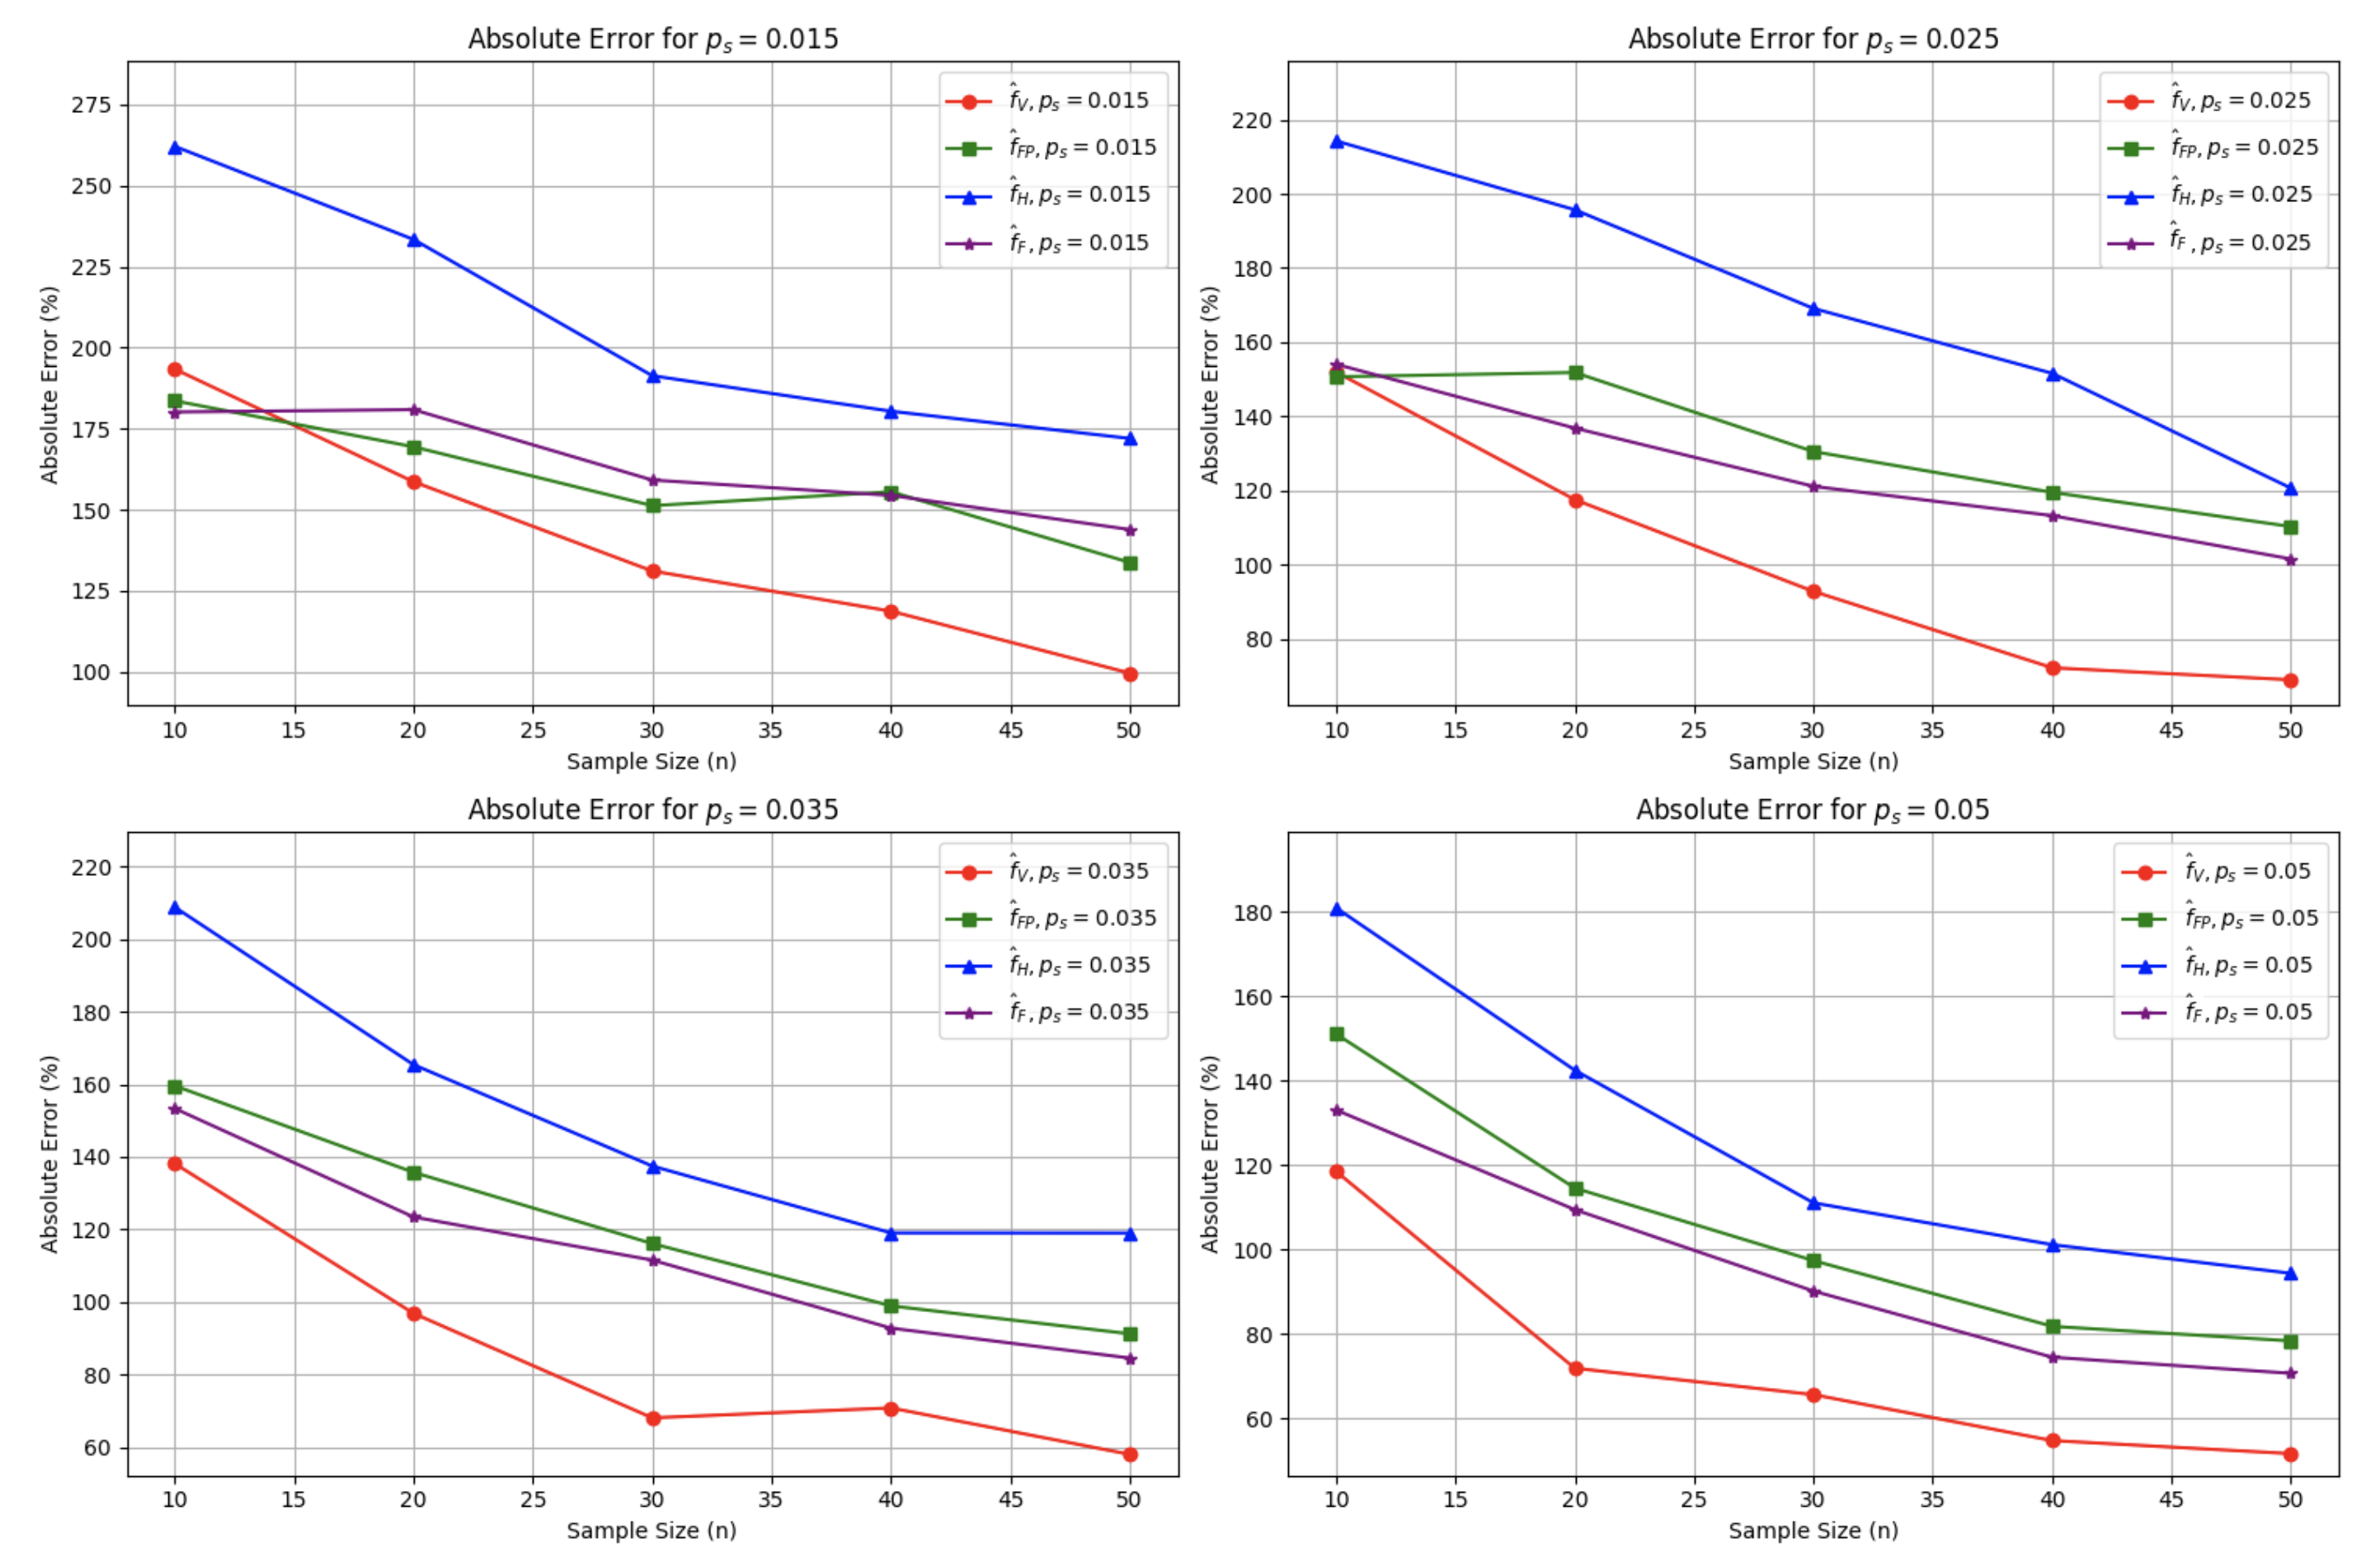
\includegraphics[scale=0.33]{estimator_performance_strong_monte500.png}
    \caption{Performance of the estimator using 500 Monte Carlo samples.}
    \label{fig:estimator_performance}
\end{figure}

The graphs in Figure 1 illustrate the absolute error percentages of four estimators—the vanilla estimator ($\hat{f}V$), the friendship-paradox-based estimator ($\hat{f}{FP}$), the hybrid estimator ($\hat{f}_H$), and the Fotouhi estimator ($\hat{f}_F$)—across varying sample sizes ($n$) for different values of $p_s$ (0.015, 0.025, 0.035, and 0.05). Each graph corresponds to a specific $p_s$ value, representing the probability of a node sharing information in the network. Smaller errors indicate better performance, as the estimators more accurately approximate the true average exposure.

Across all scenarios, the vanilla estimator consistently achieves the lowest absolute error, particularly at larger sample sizes. This aligns with its design as a simple and unbiased estimator, which benefits from direct sampling of nodes. However, its performance degrades at smaller sample sizes, especially for highly skewed networks, where the estimator's high variance becomes evident.

The friendship-paradox-based estimator shows intermediate performance. It outperforms the vanilla estimator in scenarios with small sample sizes and low $p_s$ values, leveraging the structural advantage of high-degree nodes in the network. However, its error stabilizes at a higher value compared to the vanilla estimator as sample sizes increase, reflecting the trade-off introduced by its inherent bias.

The hybrid estimator, one of our proposed methods, exhibits relatively high errors compared to the other estimators. While it aims to balance the strengths of the vanilla and friendship-paradox-based approaches, it does not achieve competitive performance. Its higher error values suggest that the weighting scheme used in its design may require further refinement to improve its effectiveness in diverse network settings.

The Fotouhi estimator, our other proposed method, demonstrates significant promise. While it does not outperform the vanilla estimator, it consistently achieves lower errors than the friendship-paradox-based estimator across all sample sizes and $p_s$ values. Notably, its performance improves as $p_s$ increases and sample size grows, indicating its potential for scenarios with higher sharing probabilities and larger datasets. This suggests that the Fotouhi estimator, by incorporating network-level quality corrections, is effective at addressing the systemic biases present in heterogeneous networks.

Overall, the results indicate that while the vanilla estimator remains the most accurate in terms of absolute error, the Fotouhi estimator is competitive and outperforms the friendship-paradox-based estimator under many conditions. These findings highlight the potential of our proposed method to serve as a robust alternative, particularly in networks where understanding quality-driven biases is critical. Future work could further enhance the hybrid estimator's design to better capture the complementary strengths of the other estimators.

\section{Future Work}

There are several directions that we can take to expand on this work. One clear next step is to test the hybrid estimator and the Fotouhi estimator on more real-world networks with different structures. For example, networks with varying levels of clustering or assortativity could reveal how well these methods perform in different settings. Another idea is to apply these estimators to networks that change over time, such as social networks where connections and information spread evolve. This could help us understand how these methods work in real-time scenarios.

Another area of improvement is to determine the best way to choose the parameter \( \alpha \) in the hybrid estimator. Currently, \( \alpha \) is set manually, but its ideal value likely depends on the structure of the network, such as how connected or spread out it is. Developing a simple, data-driven way to pick \( \alpha \) could make the hybrid estimator easier to use and more effective across different networks.

We can also think about expanding the NNQDD and NQP ideas to include more factors beyond just degree and quality. For example, adding time or location information could make these estimators more useful for networks where timing or geography plays a big role, such as traffic or event planning. Similarly, exploring how these methods could work in networks with multiple types of connections, such as personal and professional relationships, could make them more broadly applicable.

Finally, it is worth looking at ways to make sampling more efficient. While the friendship paradox-based estimator and hybrid estimator reduce some of the problems with random sampling, they still rely on information like the network’s average degree, which might not be easy to get access to in very large networks. Developing faster and more scalable sampling methods, like grouping similar nodes or using adaptive sampling, could make these estimators better suited for large-scale applications, like tracking misinformation or studying social media trends.

\nocite{*}
\printbibliography

\end{document}
